\chapter{State of the Art}\label{sec:chap:2}

For the last 40 years society has been living the third industrial revolution, better known as the digital age. Telecommunications and technological innovations are transforming the way people live and work, one way these innovations have impacted society is by allowing users to connect cheaper and quicker internationally, making it easier to share ideas than ever before. 
The ever-growing number of bots assisting humans has allowed companies to automate more and more, relieving people from the most boring of jobs, this has resulted in a higher demand for higher educated workers specially in computer science and other engineering areas. 
As you can see in the graph below, people are becoming more interested in these areas. This helps further develop these technologies as the more people interested, the more ideas are shared and more progress is done.\\

\begin{center}
	\begin{figure}[h!]
		\centering
		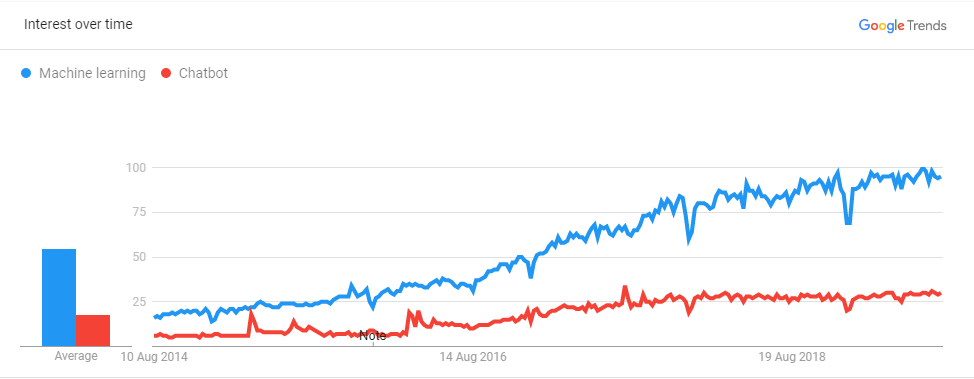
\includegraphics[scale=0.6]{./images/3-mach-chat-trend}
		\caption{Global Trends for Machine Learning and Chatbots}
		\label{global-trends-mach-chat}
	\end{figure}
\end{center}

In this chapter the background for the technologies that were used in the project will be explained. \\

\section{Artificial Intelligence}\label{sec:chap3_ai}
As Andrew Ng, a professor from Stanford said, AI is the new electricity, in a certain way the same as electricity changed many industries, AI is set to revolutionize the world. But before explaining further, let’s explain what Artificial Intelligence is. Based on Encyclopaedia Britannica’s definition, AI is the ability for digital computers of performing tasks commonly associated with intelligent beings.  There are two main ways of classifying AI:\\
\begin{itemize}
	\item {\textbf{Type 1:}
		\begin{itemize}
			\item {\textbf{Strong AI:} This is an AI that thinks just like a human. Currently there are no examples of this happening, but its development has accelerated innovations in AI.}
			\item {\textbf{Weak AI:} Build machines that do things like humans but without an understanding of how the human brain works. It is where a machine only is able of doing one task.}
		\end{itemize}
	Companies normally develop a fusion between these two types where machines have a partial understanding of how humans work to do tasks.\\
	}
	\item {\textbf{Type 2:}
		\begin{itemize}
			\item {\textbf{Reactive Machines:} One of the more basic types of Artificial Intelligence. It can’t use past information to do future actions. It focuses more on rules than actual knowledge.}
			\item {\textbf{Limited Memory:} In this case the AI can use past information to do future actions. This design for AI has been integrated in autonomous vehicles, where the car stores information of what occurs in its surroundings. This functionality is used also in chatbots to maintain a contextual idea of the conversation as the machine stores relevant information to make it more human-like.}
			\item {\textbf{Theory of Mind:} This is where a machine can understand and interpret human emotions, beliefs, thoughts, etc. By understanding what makes us human it can be able to socially interact with them. This would be the next level for chatbots, now the machine can extract a person’s emotion by the words and tone spoken with and respond differently based on that, but still has a way to go to understanding humans.}
			\item {\textbf{Self-awareness:} Still in the science fiction stage where a machine is conscious, intelligent and aware, basically a human being. If human kind reaches this point in AI, it would be a huge milestone for the field but will also raise many questions.}
		\end{itemize}
	}
\end{itemize}

Many people confuse Artificial Intelligence with machine learning, but this is wrong, machine learning is a part of AI, many other areas encompass the whole of AI. To visualize this easier the image before shows you how 	this areas are divided.\cite{ai}\\

\begin{center}
	\begin{figure}[h!]
		\centering
		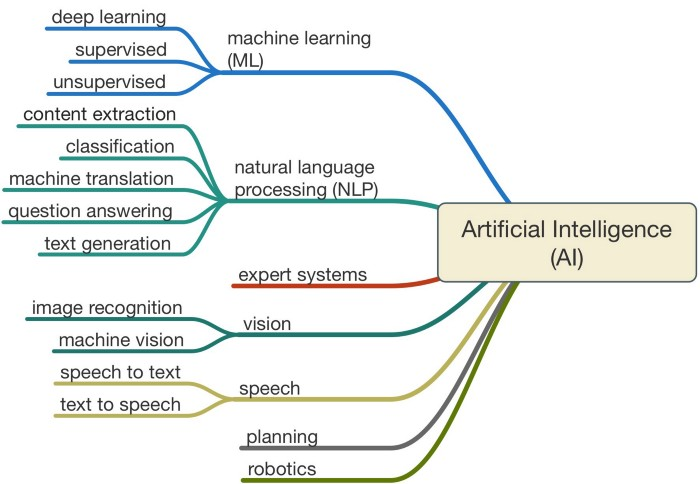
\includegraphics[scale=0.5]{./images/3-ai-areas}
		\caption{Areas in Artificial Intelligence}
		\label{ai-areas}
	\end{figure}
\end{center}

For this project the main areas that were used from AI are Machine Learning and Natural Language Processing. For a final product, speech would be an upgrade to the project to make it able to interact through voice with the user.\\

\begin{itemize}
	\item {\textbf{Machine Learning:} For this project we use supervised training where the bot has conversations with a trainer that tells what the bot should do based on what the user says.}
	\item {\textbf{Natural Language Processing:} Even though many of the tools provided are integrated in Rasa, several tools where used for the bot to work in the initial iteration of the chatbot and still requires tweaking with Rasa.\\
		
		\begin{itemize}
			\item {\textbf{Content Extraction:} This is where valuable information is extracted from what the user says, this can be what can of training they are seeking, at what time they want to be reminded to take their measurements or when the user was born. This is done by using regular expressions or by using lists with synonyms, depending of what type of info is extracted.}
			\item {\textbf{Classification:} Depending on what the user says, the bot must understand what his intentions are, this is done by training the bot with training phrases that reflect what does the user want and associating it with an intention, after training a model, the bot is able to distinguish between different intentions. Before training the bot, human phrases must be translated to something the machine can understand.}
		\end{itemize}
			}
\end{itemize}


\section{Chatbots}\label{sec:chap3_ai}
A chatbot is a software based on AI that simulates a human conversation with a user. This is done through messaging applications such as Telegram, Facebook, websites or company’s messaging software.\\

Chatbots have been slowly but steadily been incorporated into people’s lives, from basic robo-calls to natural speaking bots used in customer service. Virtual assistants such as Google or Alexa, that are constantly getting feature updates making bigger the number of things they can do, such as ordering pizza or getting a booking for a restaurant. These improvements have to do with many of the technologies involved, that have improved greatly. We will explain below the different components in a chatbot and how its architecture has evolved.\\

\subsection{Messaging Platform}\label{sec:chap3_cha_mes_pla}
The messaging app is where the user interacts with the chatbot. As mentioned previously there are several ways of communicating with the chat bot, it can be written or spoken. Depending on how the user talks with the chat bot there will be additional processing, because if the user uses spoken language it must be transcribed for the machine to understand.\\

\subsection{Natural Language Processor}\label{sec:chap3_cha_nlp}
The Natural Language Processor is the step where the bot does most of the work. When the message is received it goes through a series of conversions.\\

\begin{itemize}
	\item {\textbf{Speech to Text:} This is needed only when the message sent from the user is in voice format, such as the virtual assistants solutions provided by Google or Amazon, although this can also be included in applications where voice messages functionality is available.}
	\item {\textbf{Language Detection:} This is a way of building a multilingual chatbot without the need of building different models for every language. The issue is how to get the translation, there is a well-known API from google that provides this functionality for a price. A way to reduce costs can be to have a cache store the most frequent translations.}
	\item {\textbf{Tokenizing:} In this step what the bot does is separate the phrases in independent words, it is also important for the bot to understand what each word is, if it is a noun, verb, adjective or an adverb. Also, it must discard all redundant words that don’t provide any additional information.}
	\item {\textbf{Stemming:} This consists in simplifying the words in the phrase in order to have a much simpler vocabulary for the bot to understand, this is done by eliminating verb conjugations or keeping the stem of the word. In the image below there is a more in detail example of what stemming is.\cite{cha-stem}}
	
	\begin{center}
		\begin{figure}[h!]
			\centering
			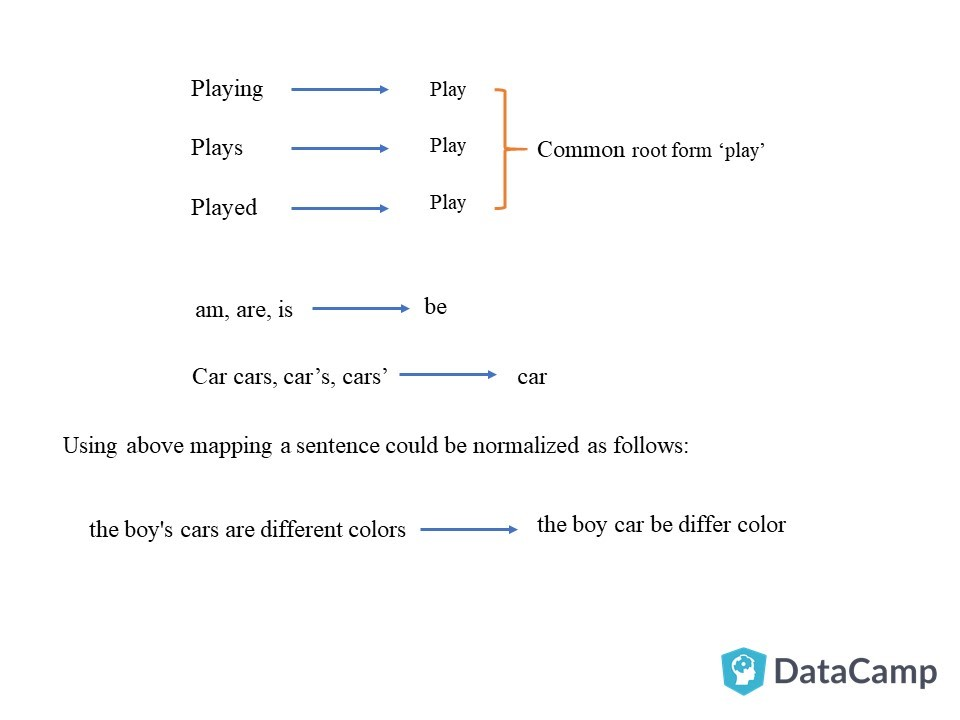
\includegraphics[scale=0.7]{./images/3-chatbot-stemming}
			\caption{Stemming Examples}
			\label{cha_stem}
		\end{figure}
	\end{center}

	\item {\textbf{Word to number:} The bot in at this point translates the tokenized and stemmed words into numbers the bot can understand, this is done in two steps.\\
			\begin{itemize}
				\item {\textbf{Word Identifier:} In this step what the bot does is convert each word with a numerical identifier. In this way, for example all the hello’s will be number 1. This helps the bot in the next step.}
				\item {\textbf{Term Frequency:} Here what the bot does is check the frequency of certain words in the training data. This will be used to help classify as some words are more frequent in some intents more than in others.}
			\end{itemize}	
		}
	\item {\textbf{Intent detection:} Based on the frequency words show up on the user’s message the bot can predict what the user’s intention is.}
	\item {\textbf{Entity Extraction:} Once the intent is predicted the next step is extracting the information that is relevant to that intent, in case of setting a reminder for example it is important for the bot to understand at what time does the user wants to be reminded.\\
	This can be done in several ways:\\ 
			\begin{itemize}
				\item {Regular expressions to extract information that comes in certain formats.}
				\item {Lists for finite proper names, like cities or countries.}
				\item {By adding many examples of the data that you want the bot to extract.}
				\item {Filling the missing information with user relevant info extracted in previous occasions.}
				\item {Asking the user for the missing information.}
			\end{itemize}
		}
	\item {\textbf{Response:} After extracting all the relevant information from the user’s message create a response that answers the user’s request and perform whichever action needs to be performed.}
\end{itemize}

\subsection{Profiler}\label{sec:chap3_cha_pro}
The profiler is an extension of the chatbot that allows it to become much more intuitive and natural with the conversations. What the profiler does is gather information from the user through their previous conversations, then uses that info to give context to the user’s requests or fills out missing information based on the user’s preferences.\\

For example, in this project when the user asks to be reminded to take his measurements at 8 am, the bot will extract that information for future occasions. If after that interaction the user asks to be reminded the next day the bot will automatically use the hour extracted from the previously without asking the user for that information.\\

\begin{center}
	\begin{figure}[h!]
		\centering
		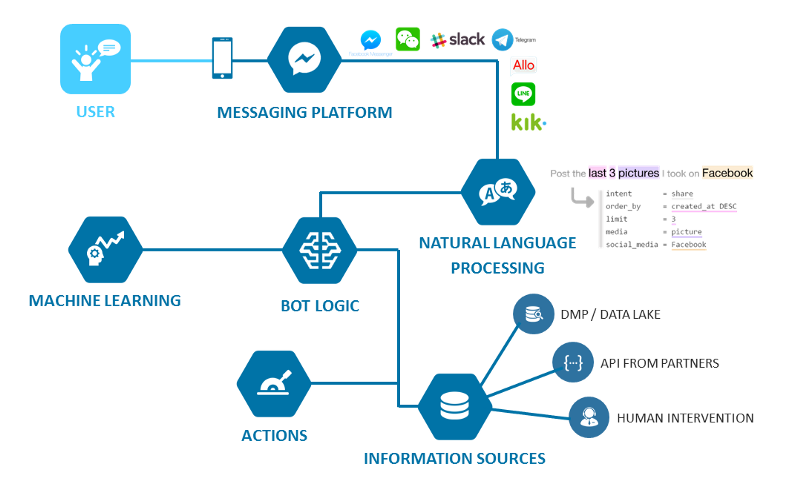
\includegraphics[scale=0.6]{./images/3-cha-struct}
		\caption{Chatbot Architecture}
		\label{cha_struct}
	\end{figure}
\end{center}

\section{Platforms}\label{sec:chap3_plat}

There are many platforms to build chatbots, with their own features. Below there is a table of the difference between several solutions. In this section we will talk about some of them and what differences each have.\\


\begin{table}[h!]
	\centering
	\resizebox{\linewidth}{!}{%
		\begin{tabular}{|c|c|c|c|c|} 
			\hline
			\rowcolor[rgb]{0.753,0.753,0.753} Bot Name                                                               & Features                                                                                                                                                                                                                                           & Technical Details                                                                                                                                                                           & License                                                                                                                                  & Channel                                                        \\ 
			\hline
			\begin{tabular}[c]{@{}c@{}}IBM Watson \\Conversation Service \end{tabular}                               & \begin{tabular}[c]{@{}c@{}}Has three main components: \\Intents, \\Entities, \\Dialog\\ \\ Analysis, to detect what\\~messages confuse the bot \end{tabular}                                                                                       & \begin{tabular}[c]{@{}c@{}}Built on a neural network \\(one billion Wikipedia words). \end{tabular}                                                                                         & \begin{tabular}[c]{@{}c@{}}Free, priced \\per message,\\ \\ Contact required \\for enterprise \end{tabular}                              & \begin{tabular}[c]{@{}c@{}}Voice\\ Image\\ Text \end{tabular}  \\ 
			\hline
			Wit.ai                                                                                                   & \begin{tabular}[c]{@{}c@{}}Home automation\\ \\ Wearables\\ \\ Hardware \end{tabular}                                                                                                                                                              & \begin{tabular}[c]{@{}c@{}}Allows to use:\\ \\ Entities\\ Intents\\ Context\\ Actions \end{tabular}                                                                                         & Free                                                                                                                                     & \begin{tabular}[c]{@{}c@{}}Voice\\ Text \end{tabular}          \\ 
			\hline
			Rasa                                                                                                     & \begin{tabular}[c]{@{}c@{}}Interactive Learning\\ \\ Stories \end{tabular}                                                                                                                                                                         & \begin{tabular}[c]{@{}c@{}}Modular Pipeline to \\design what best fits for you \end{tabular}                                                                                                & Open Source                                                                                                                              & Text                                                           \\ 
			\hline
			Dialogflow                                                                                               & \begin{tabular}[c]{@{}c@{}}Intuitive Platform\\ \\ Pretrained packages \\from Google\\ \\ Chit Chat built in \end{tabular}                                                                                                                         & \begin{tabular}[c]{@{}c@{}}Neural Network\\ \\ Black box \end{tabular}                                                                                                                      & \begin{tabular}[c]{@{}c@{}}Free\\ Enterprise \end{tabular}                                                                               & \begin{tabular}[c]{@{}c@{}}Voice\\ Text \end{tabular}          \\ 
			\hline
			\begin{tabular}[c]{@{}c@{}}Microsoft Language \\Understanding\\~Intelligent Service (LUIS) \end{tabular} & \begin{tabular}[c]{@{}c@{}}All LUIS applications are \\centered around a \\domain-specific topic or\\ content related.\\ \\ Active learning.\\ \\ You can use pre-existing, \\world-class, pre-built \\models from Bing and Cortana. \end{tabular} & \begin{tabular}[c]{@{}c@{}}LUIS offers a set of \\programmatic REST APIs \\that can be used by\\ developers to automate \\the application creation process. \end{tabular}                   & \begin{tabular}[c]{@{}c@{}}Free\\{[}10.000 Transactions]\\Paid\\{[}1,50\$1.000 transactions]\\{[}4,50\$ 1.000transactions]~\end{tabular} & \begin{tabular}[c]{@{}c@{}}Voice\\ Text \end{tabular}          \\ 
			\hline
			Pandorabots                                                                                              & \begin{tabular}[c]{@{}c@{}}AIML (Artificial Intelligence \\Markup Language) \\ \\ Includes A.L.I.C.E. \end{tabular}                                                                                                                                & \begin{tabular}[c]{@{}c@{}}The Pandorabots API allows \\you to integrate our bot \\hosting service and\\ \\ natural language \\processing engine into \\your own application. \end{tabular} & \begin{tabular}[c]{@{}c@{}}Free\\Developer [19\$/month]\\Pro [199\$/month]\\~Enterprise [Sales]~ ~~\end{tabular}                         & Text                                                           \\
			\hline
		\end{tabular}
	
	}
\label{cha_diff}
\caption{Differences between different chatbot solutions}
\end{table}
 

\subsection{DialogFlow}\label{sec:chap3_pla_rasa}



\subsection{Rasa}\label{sec:chap3_pla_dia}

\begin{center}
	\begin{figure}[h!]
		\centering
		
\includegraphics[scale=0.4]{./images/3-rasa-log}
		\caption{Rasa Logo}
		\label{rasa_logo}
	\end{figure}
\end{center}

\cite{rasa}